\chapter{Aplikacija}

	Aplikacija je skup alata razvijenih za praćenje znanja, clusteriranje zadataka u koncepte, preporuke zadataka s obizrom na povijest rješavanih zadataka, izgradnje grafova koji pokazuju odnos koncepata i pitanja.
	
	
	\begin{comment}
		Knowledge tracing
		- bayesian knowledge tracing- input su dataset za određeni "ispit",pragovi za cutoff,gauss,bkt -potencijalno slideri sa listenerima pa se prema tome mijenja graf?
			-output: graf koji pokazuje odnos koncepata (usmjereni graf)
			-prvo treba proci vrijeme dok se izracunaju parametri za bkt -bilo bi dobro imati mogucnost sejvanja generiranih parametara u neki pikl?
			-kod procesuiranja google formsa u dataset treba dati pravilan redoslijed naziva koncepata
		OGRANIČENJA- u datasetu svi korisnici moraju rijesiti sve zadatke i to istim redoslijedom
		
		ExRec-
		KT dio- moguce izvrsiti samo jednom za neki dataset i onda spremiti parametre u neki pikl koji se moze kasnije kako bi bilo brze
		Izracun matrice relevantnosti preko SAKT-a se isto moze jednom izvrsiti i onda se objekt klase "PersonalCandidates" ili sama matrica mogu spremiti kao pikl i koristiti kasnije, mozda bolje matrica jer za PersonalCandidates postoje varijabilni argumenti
		PersonalCandidates- ima mogucnost razlicith normalizacijskih funkcija i funkcija praga te same vrijednosti praga

		Recommmendation system ima ulaz parametre dobivene iz kt dijela, student traces (tu bi moglo staviti da se upisu zadaci i tocno/netocno ili da se ucita iz nekog fajla pa da se onda da preporuku i opciju da li da se radi samo sakt preporuka ili sakt + rs)
		
		Clustering
		-k-mediods - uz input min,max broj koncepata i ulazni dataset daje procjenu koliko zapravo koncepata ima
					-uz dani broj koncepata clusterira pitanja u različite koncepte
					-ograničenja su jednaka kao za bkt
					
		-zvonimir
		
		-bkt izgradnja grafa gdje se pitanja gledaju kao koncepti (to bi vjerojatno trebalo preraditi i trebalo bi se igrati sa parametrima)
			-trenutno se za izgradnju prima googleforms file, treba generalizirati za opceniti dataset
			-treba promijena funkcija get_student_concept_mastery
		-pomocne skripte- obrada google formsa, generiranje umjetnog dataseta
		
	\end{comment}

Prilikom izrade aplikacije potrebno je ostvariti da se frontend i backend mogu bez poteškoća izvršavati na bilo kojem uređaju, ne samo na lokalnom. Garancija da će izvršavanje prolaziti bez problema je istovjetnost cloud okruženja lokalnom okruženju. Kako bi se smanjio jaz između cloud i lokalnog okruženja, potrebno je cloud provideru definirati što su potrebe aplikacije. No, cloud provider može imati mnogo developera pa zbog jedinstvenosti nudi različite pakete. Variraju između korištenja virtualnog stroja i omogućavanja izvršavanja aplikacije u statičnom okruženju. Docker nudi fleksibilan standard koji omogućuje izvršavanje softveta na cloudu jednako kao lokalno. Više je od obične tehnike virtualizacije: moguća je izgradnja, \textit{deployment} i upravljanje kontejnerima. Izolirana je platforma koja obuhvaća sve što je potrebno za izvođenje specifične aplikacije. Srž Dockera je \textit{image} sustav. \textit{Image} je kombinacija datotečnog sustava i parametara. Docker sustav sastoji se od Docker klijenta (API-ja), daemona/enginea (pozadinskog procesa koji dohvaća i pokreće \textit{image} i huba (repozitorija svih \textit{imagea)}.\newline
Deployment aplikacije u cloud izvršava se pomoću Heroku. 

\section{Instalacija Dockera}
Sama instalacija Dockera na operacijskom sustavu Windows 8.1. pokazala se izazovnom pa je odlučeno ostaviti zapis o suočavanju s problemima i ukazati na moguća rješenja. \newline
Prilikom instalacije Docker Toolbox-a, u uputama je navedeno kako nije potrebno instalirati VirtualBox ako već postoji na računalu. No, javila se greška prikazana na slici ~\ref{fig:docker1}.\pagebreak

\begin{figure}[!htb]
	\centering
	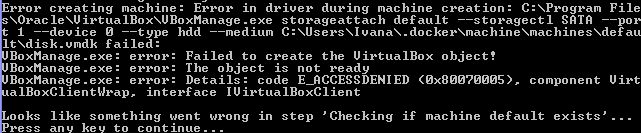
\includegraphics[scale=0.8]{docker1.jpg}
	\caption{Docker greška - VirtualBox}
	\label{fig:docker1}
\end{figure}

Ispravljena je deinstalacijom VirtualBox-a i Docker Toolbox-a te reinstalacijom Docker Toolbox-a uz označene sve \textit{requiremente}, pa i VirtualBox.\newline
Nadalje, javljala se greška o onemogućenosti virtualizacije (slika ~\ref{fig:docker2}), iako je u BIOS-u virtualizacija bila omogućena. StackOverflow je kao mogućnost rješenja nudio onemogućavanje Microsoft Hyper-V-a (kreatora virtualnih strojeva na x86-64 Windows sustavima), no postojanje istog uopće nije zamijećeno na računalu.  VirtualBox je za to vrijeme tvrdio kako CPU ne odgovara kernelu (slika ~\ref{fig:docker4}).

\begin{figure}[!htb]
	\centering
	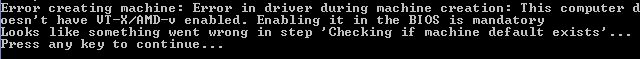
\includegraphics[scale=0.8]{docker2.jpg}
	\caption{Docker greška virtualizacije}
	\label{fig:docker2}
\end{figure}

\begin{figure}[!htb]
	\centering
	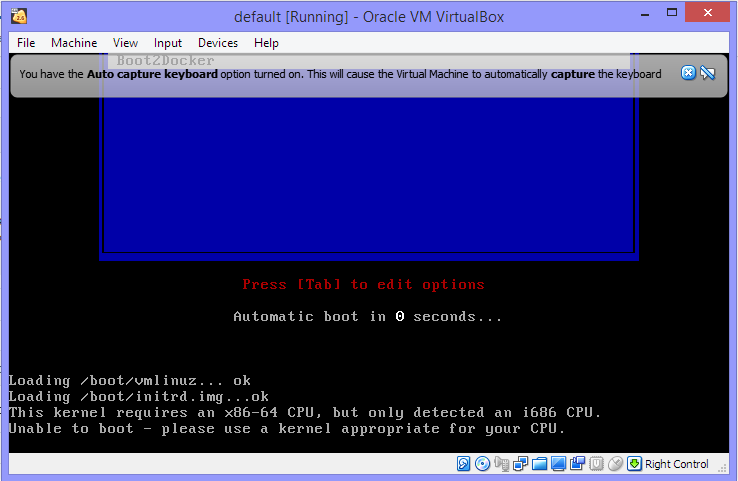
\includegraphics[scale=0.7]{docker4.png}
	\caption{Docker greška virtualizacije}
	\label{fig:docker4}
\end{figure}

Ponovnim odlaskom u BIOS i provjerom omogućene virtualizacije te restartom računala, problem je nestao.

Sljedeća greška (slika ~\ref{fig:docker3}) bila je vezana uz pokretanje Docker enginea. 

\begin{figure}[!htb]
	\centering
	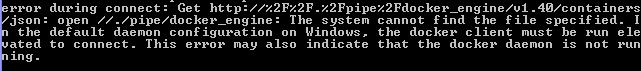
\includegraphics[scale=0.8]{docker3.jpg}
	\caption{Docker greška daemona}
	\label{fig:docker3}
\end{figure}

Ponovim otvaranjem Toolbox-a, javila se i greška "Error checking TLS connection: Host is not running", što je isto riješeno resetom računala.

\section{Heroku}
Gradivni blokovi svake Heroku aplikacije su tzv. \textit{dynosi}, izolirani i virtualizirani kontejneri dizajnirani da izvršavaju kod prema specifikacijama korisnika.\newline

Kao moguće ograničenje Heroku identificirana je činjenica da nakon što se na isti račun pokuša postaviti šesta aplikacija ili pokuša koristiti više od jednog \textit{dynosa}, dobije se obavijest "You've reached the limit of 5 apps for unverified accounts. Delete some apps or add a credit card to verify your account." \newline
Smatra se da je potrebno moći pouzdano identificirati i kontaktirati korisnike Heroku u slučaju poteškoća.

\section{Poveznice}
\url{https://milanwittpohl.com/projects/tutorials/Full-Stack-Web-App/dockerizing-our-front-and-backend} \newline
\url{https://milanwittpohl.com/projects/tutorials/Full-Stack-Web-App/deployment-in-the-cloud-using-heroku} \newline
\url{https://docs.docker.com/get-started/part2/} \newline
\url{https://medium.com/@wkrzywiec/how-to-run-database-backend-and-frontend-in-a-single-click-with-docker-compose-4bcda66f6de} \newline
\url{https://www.heroku.com/deploy-with-docker} \newline
\url{https://devcenter.heroku.com/articles/container-registry-and-runtime} \newline
\url{https://devcenter.heroku.com/articles/build-docker-images-heroku-yml}\newline
\url{https://devcenter.heroku.com/articles/limits#maximum-number-of-apps}\newline

	 
